\documentclass[border=10pt]{standalone}
\usepackage{pgfplots}
\pgfplotsset{compat=1.18}
\begin{document}
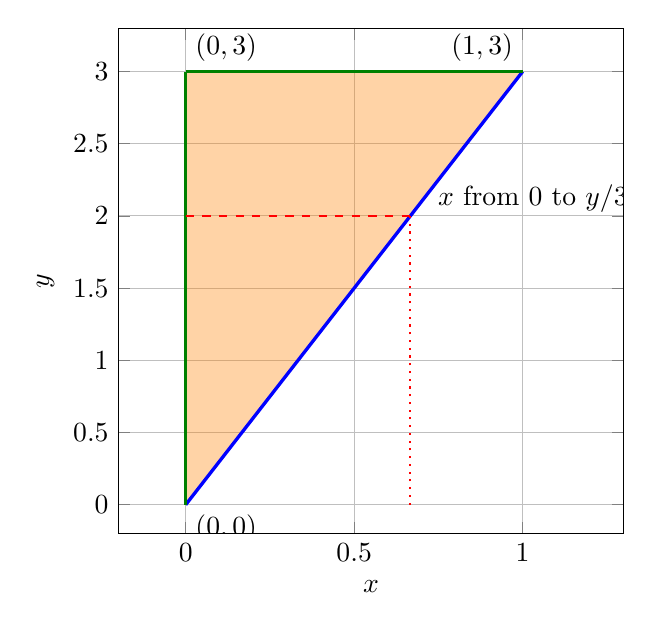
\begin{tikzpicture}
\begin{axis}[
    axis lines=box,
    xlabel=$x$, ylabel=$y$,
    xmin=-0.2, xmax=1.3,
    ymin=-0.2, ymax=3.3,
    width=8cm, height=8cm,
    grid=major,
    enlargelimits=false,
    xtick={0,0.5,1},
    ytick={0,0.5,1,1.5,2,2.5,3},
]
% shaded projection region (triangle)
\addplot[fill=orange, opacity=0.35, draw=none]
    coordinates {(0,0) (1,3) (0,3)} \closedcycle;
% boundaries
\addplot[blue, very thick, domain=0:1, samples=2] {3*x};
\addplot[green!50!black, very thick] coordinates {(0,0) (0,3)};
\addplot[green!50!black, very thick] coordinates {(0,3) (1,3)};
% typical horizontal strip at y=2
\addplot[red, thick, dashed] coordinates {(0,2) (2/3,2)};
\addplot[red, dotted, thick] coordinates {(2/3,0) (2/3,2)};
\node[right] at (axis cs:0.72,2.12) {$x$ from $0$ to $y/3$};
% vertices
\node[below right] at (axis cs:0,0) {$(0,0)$};
\node[above right] at (axis cs:0,3) {$(0,3)$};
\node[above left] at (axis cs:1,3) {$(1,3)$};
\end{axis}
\end{tikzpicture}
\end{document}
